\chapter{Design}
\label{cap:design}

Il presente capitolo illustra la progettazione di \textbf{CiboAmico}: dapprima la vista di analisi (VOPC) del caso d'uso core, quindi il diagramma delle classi di progettazione, i pattern GoF applicati e la modellazione comportamentale (activity, sequence e state) per il caso d'uso \textbf{Ordina un Prodotto}.

\section{View of Participating Classes (VOPC)}
\label{sec:vopc}

Il \textbf{VOPC} è il diagramma delle classi di analisi che mostra \emph{solo} i partecipanti del caso d'uso \textbf{Ordina un Prodotto} (UC-04). L'architettura segue il pattern \textbf{Boundary--Control--Entity}:
\begin{itemize}
    \item ogni caso d'uso possiede \textbf{esattamente un} controller applicativo;
    \item la boundary scambia dati con il controller esclusivamente tramite \textbf{Bean} (regola bean-only): nessuna entity raggiunge la view;
    \item il controller è \textbf{stateless}: l'utente corrente è passato dalla view e risolto dalla sessione;
    \item la logica risiede nelle entità (GRASP Information Expert).
\end{itemize}

La tabella~\ref{tab:vopc} riassume le classi partecipanti di tutti i casi d'uso implementati (tracciabilità reale sul codice): una boundary per nodo di interazione, un controller per caso d'uso e le entity manipolate.

\begin{table}[H]
    \centering
    \footnotesize
    \resizebox{\textwidth}{!}{
    \begin{tabular}{@{}llll@{}}
        \toprule
        \textbf{Use Case} & \textbf{Boundary} & \textbf{Control} & \textbf{Entity / Bean}\ \\ \midrule
        UC-01 Dispensa & \texttt{InventarioView} & \texttt{GestisciInventarioController} & \texttt{ProdottoInventario}, \texttt{Prodotto}, \texttt{ProdottoBean}\\ \midrule
        UC-02 Ricette compatibili & \texttt{RicetteView} & \texttt{TrovaRicetteController} & \texttt{Ricetta}, \texttt{ProdottoInventario}, \texttt{RicettaBean}\\ \midrule
        UC-03 Lista spesa & \texttt{ListaSpesaView} & \texttt{GestisciListaSpesaController} & \texttt{Ricetta}, \texttt{Ingrediente}, \texttt{ProdottoInventario}\\\midrule
        UC-04 Ordina Prodotto & \texttt{MarketplaceView} & \texttt{OrdinaProdottoController} & \texttt{Ordine}, \texttt{VoceOrdine}, \texttt{Prodotto}, \texttt{BuonoPromozionale}, \texttt{Utente}\\ \midrule
        UC-05 Catalogo venditore & \texttt{CatalogoVenditoreView} & \texttt{GestisciCatalogoVenditoreController} & \texttt{Prodotto}, \texttt{RuoloVenditore}\\ \midrule
        UC-06 Ordini ricevuti & \texttt{OrdiniRicevutiView} & \texttt{GestisciOrdiniRicevutiController} & \texttt{Ordine}, \texttt{OrdineBean}\\ \midrule
        UC-07 Ricette nutrizionista & \texttt{RicetteNutrizionistaView} & \texttt{GestisciRicetteNutrizionistaController} & \texttt{Ricetta}, \texttt{Ingrediente}, \texttt{RuoloNutrizionista}, \texttt{RicettaBean}\\ \midrule
        UC-08 Approvazioni & \texttt{AdminView} & \texttt{ApprovazioneController} & \texttt{RuoloVenditore}, \texttt{Ricetta}\\ \midrule
        UC-11 Login & \texttt{LoginView} & \texttt{AutenticazioneController} & \texttt{Utente}, \texttt{UtenteBean}\\ \bottomrule
    \end{tabular}
    }
    \caption{VOPC: matrice di tracciabilità Use Case $\rightarrow$ classi partecipanti (Boundary/Control/Entity/Bean).}
    \label{tab:vopc}
\end{table}

La Figura~
ef{fig:vopc} mostra il VOPC di UC-04 secondo il modello
\emph{Boundary--Control--Entity} puro (pre-MVC): sono rappresentate solo le
classi di analisi partecipanti --- le boundary \texttt{MarketplaceView} e
\texttt{PaymentView} (a cui si collega l'attore Cliente), il control
\texttt{OrdinaProdottoController} (unico per caso d'uso) e le entity di dominio
\texttt{Ordine}, \texttt{Prodotto}, \texttt{BuonoPromozionale} e \texttt{Utente}.
Le boundary esterne \texttt{PaymentGateway} (autorizzazione pagamento, passo 6)
e \texttt{VenditoreNotifier} (notifica asincrona al Venditore) chiudono i
confronti col mondo esterno (attore Venditore a margine). Nel diagramma sono
presenti SOLO attributi strutturali rilevanti e operazioni di business, senza
getter/setter e senza dettagli implementativi (per non cadere nel
reverse engineering). I Bean/DTO e i DAO sono elementi di \emph{design-level}
(regola bean-only al confine, introdotta in progettazione): sono quindi
mostrati nel class diagram di progettazione e non in questa vista di analisi.

\begin{figure}[H]
    \centering
    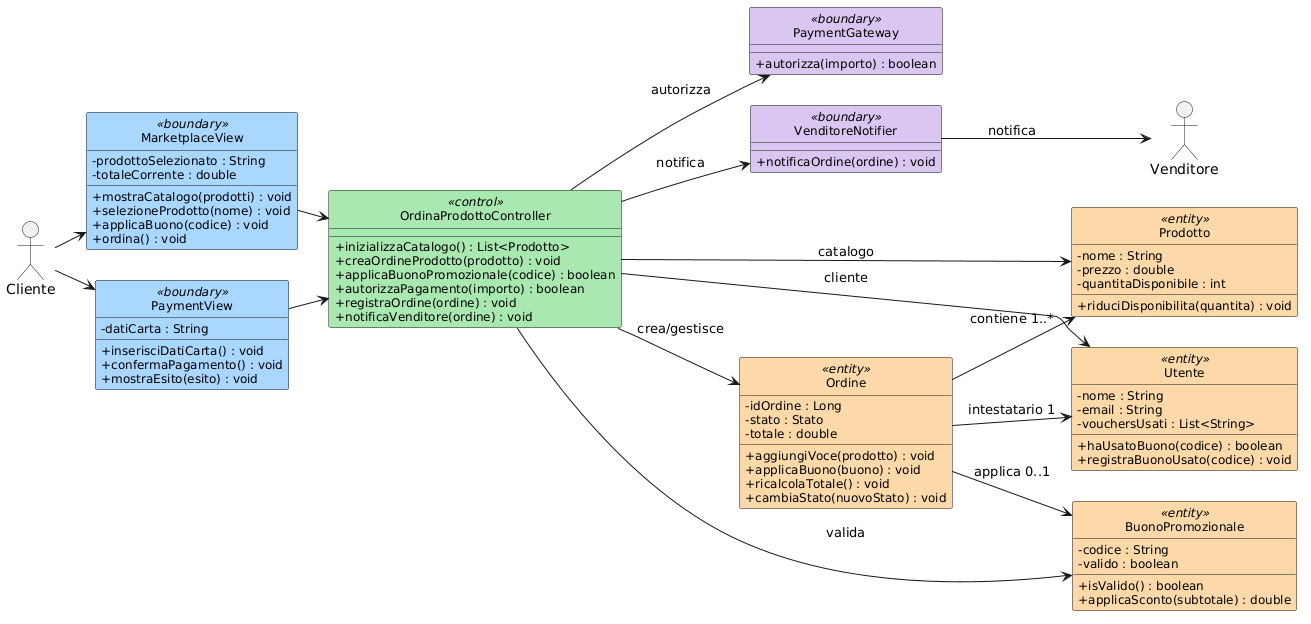
\includegraphics[width=\textwidth]{figures/vopc_uc04.png}
    \caption{VOPC (analisi BCE pura) del caso d'uso Ordina un Prodotto: solo
    Boundary, Control ed Entity con attributi rilevanti e operazioni di
    business; attore Cliente/Venditore a margine, Bean/DAO a design-level.}
    \label{fig:vopc}
\end{figure}



